\section{Fits}
\label{s:fits}

Data presented in fig. 4 from \cite{PhysRevLett.105.167202}
was fit
\footnote{
  Fits done using the scipy-data\_fitting Python package:
  \href{https://github.com/razor-x/scipy-data_fitting}{github.com/razor-x/scipy-data\_fitting}.
  Code used to create the fits can be found at
  \href{https://github.com/razor-x/spin-lifetime-analysis}{github.com/razor-x/spin-lifetime-analysis/tree/aps}.
  Code used to generate the figures can be found at
  \href{https://github.com/razor-x/aps-spin-lifetime-plots}{github.com/razor-x/aps-spin-lifetime-plots}.
}
\cite{Hunter:2007}
to the model presented here.
The resistance of the ferromagnet \ce{Co} is computed as
$R_F = ρ_F λ_F / A_J$,
where $A_J$ is the junction area estimated at $A_J = W d$,
with $d$ between \SIrange[range-phrase={ and }]{0.5}{50}{\nano \meter}
\cite{PhysRevLett.105.167202}.

\Cref{fig:nonlocal_resistance.difference}
shows that the overall effect of including a finite $R_C$ is to increase $τ$.
Fits (a) and (b) with tunneling contacts give large
$R_C ∼ \SI{10e7}{\kilo \ohm}$ and comparable lifetimes,
while (d) with transparent contacts gives a reduced $R_C ∼ \SI{3}{\kilo \ohm}$
and a lifetime increased by a factor of two.

\begin{figure}
  \caption{
    Data in fig. 4 from \cite{PhysRevLett.105.167202}
    fit to \cref{eq:nonlocal_resistance.difference}
    with the following values: \plotDifferenceInfo.
    The contact type (tunneling or transparent)
    and the contact separation $L$ varies.
  }
  \label{fig:nonlocal_resistance.difference}
  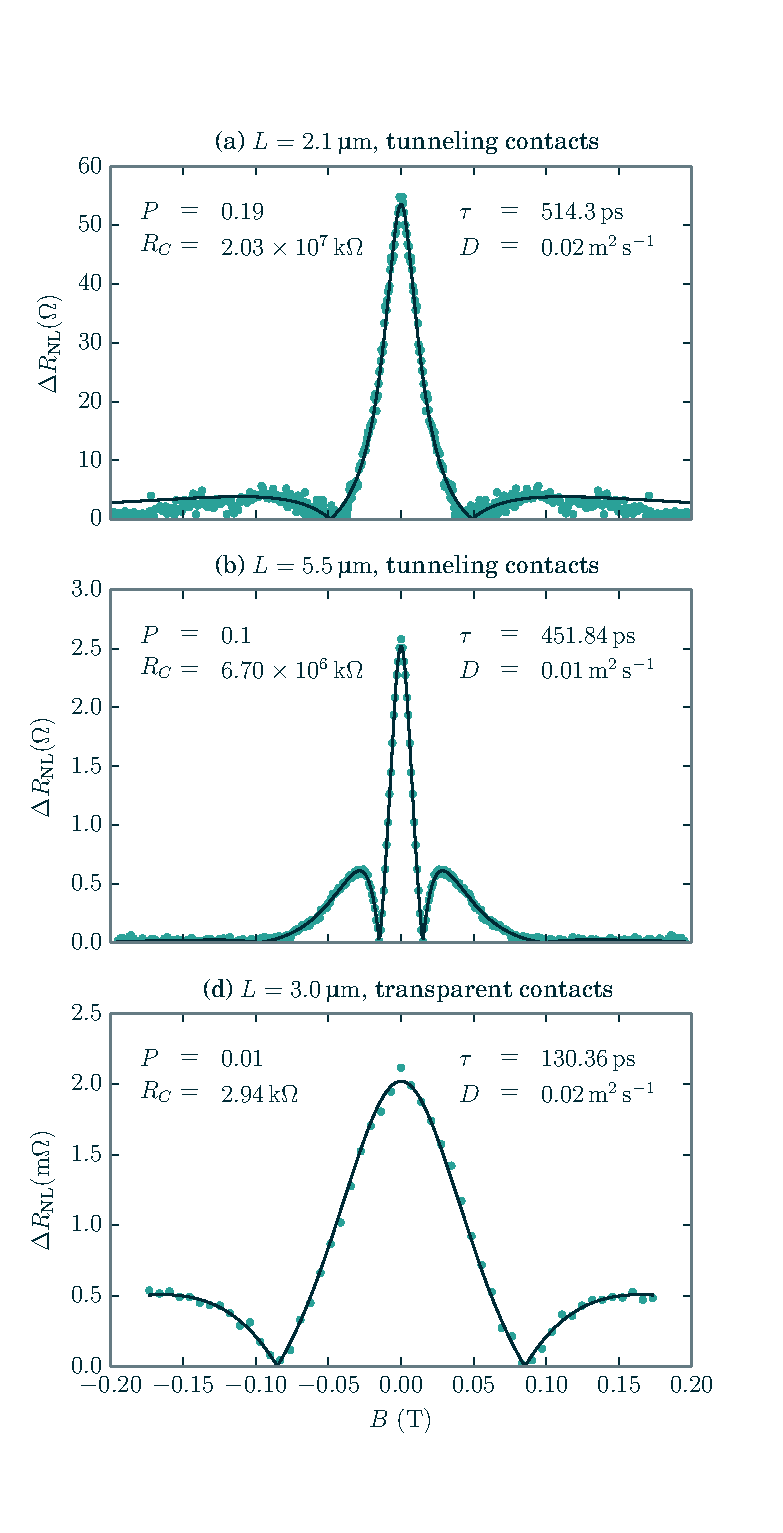
\includegraphics[width=\columnwidth]{figures/plot_difference}
\end{figure}
